%%%%%%%%%%%%%%%%%%%%%%%%%%%%%%%%%%%%%%%%%%%
%
% From a template maintained at https://github.com/jamesrobertlloyd/cbl-tikz-poster
%
% Code near the top should be fairly standard and not need to be changed
%  - except for the document class
% Code lower down is more likely to be customised
%
%%%%%%%%%%%%%%%%%%%%%%%%%%%%%%%%%%%%%%%%%%%

%%%%%%%%%%%%%%%%%%%%%%%%%%%%%%%%%%%%%%%%%%%
%
% Document class
%
% Change this if you want a different size / orientation poster etc
%
%%%%%%%%%%%%%%%%%%%%%%%%%%%%%%%%%%%%%%%%%%%

\documentclass[landscape,a0b,final,a4resizeable]{a0poster}
%\documentclass[portrait,a0b,final,a4resizeable]{a0poster}

%%%%%%%%%%%%%%%%%%%%%%%%%%%%%%%%%%%%%%%%%%%
%
% 'Basic' packages
%
% TODO - Almost certainly some are unnecessary - feel free to remove nonstandard
% packages if you think it is a good idea not to always have them
%
%%%%%%%%%%%%%%%%%%%%%%%%%%%%%%%%%%%%%%%%%%%

\usepackage{qrcode}
\usepackage{multicol}
\usepackage{color}
\usepackage{shadow}
\usepackage{morefloats}
\usepackage{cite}
\usepackage[pdftex]{graphicx}
\usepackage{rotating}
\usepackage{amsmath, amsthm, amssymb, bm}
\usepackage{array}
\usepackage{nth}
\usepackage[square,numbers]{natbib}
\usepackage{booktabs}

%%%%%%%%%%%%%%%%%%%%%%%%%%%%%%%%%%%%%%%%%%%
%
% TIKZ packages and common definitions
%
% Add extra things as per your tikz needs
%
%%%%%%%%%%%%%%%%%%%%%%%%%%%%%%%%%%%%%%%%%%%

\usepackage{a0size}
\usepackage{tikz}
\usetikzlibrary{shapes.geometric,arrows,chains,matrix,positioning,scopes,calc}
\tikzstyle{mybox} = [draw=white, rectangle]

%%%%%%%%%%%%%%%%%%%%%%%%%%%%%%%%%%%%%%%%%%%
%
% myfig
%
% \myfig - replacement for \figure
% necessary, since in multicol-environment
% \figure won't work
%
%%%%%%%%%%%%%%%%%%%%%%%%%%%%%%%%%%%%%%%%%%%

\newcommand{\myfig}[3][0]{
\begin{center}
    \vspace{1.5cm}
    \includegraphics[width=#3\hsize,angle=#1]{#2}
    \nobreak\medskip
\end{center}}

%%%%%%%%%%%%%%%%%%%%%%%%%%%%%%%%%%%%%%%%%%%
%
% mycaption
%
% \mycaption - replacement for \caption
% necessary, since in multicol-environment \figure and
% therefore \caption won't work
%
%%%%%%%%%%%%%%%%%%%%%%%%%%%%%%%%%%%%%%%%%%%

%\newcounter{figure}
\setcounter{figure}{1}
\newcommand{\mycaption}[1]{
\vspace{0.5cm}
\begin{quote}
{{\sc Figure} \arabic{figure}: #1}
\end{quote}
\vspace{1cm}
\stepcounter{figure}
}

%%%%%%%%%%%%%%%%%%%%%%%%%%%%%%%%%%%%%%%%%%%
%
% Some standard colours
%
%%%%%%%%%%%%%%%%%%%%%%%%%%%%%%%%%%%%%%%%%%%

\definecolor{camlightblue}{rgb}{0.601 , 0.8, 1}
\definecolor{camdarkblue}{rgb}{0, 0.203, 0.402}
\definecolor{camred}{rgb}{1, 0.203, 0}
\definecolor{camyellow}{rgb}{1, 0.8, 0}
\definecolor{lightblue}{rgb}{0, 0, 0.80}
\definecolor{white}{rgb}{1, 1, 1}
\definecolor{whiteblue}{rgb}{0.80, 0.80, 1}

%%%%%%%%%%%%%%%%%%%%%%%%%%%%%%%%%%%%%%%%%%%
%
% Some look and feel definitions
%
%%%%%%%%%%%%%%%%%%%%%%%%%%%%%%%%%%%%%%%%%%%

\setlength{\columnsep}{0.03\textwidth}
\setlength{\columnseprule}{0.0018\textwidth}
\setlength{\parindent}{0.0cm}

%%%%%%%%%%%%%%%%%%%%%%%%%%%%%%%%%%%%%%%%%%%
%
% \mysection - replacement for \section*
%
% Puts a pretty box around some text
% TODO - any other thoughts for what this box should look like
%
%%%%%%%%%%%%%%%%%%%%%%%%%%%%%%%%%%%%%%%%%%%

\tikzstyle{mysection} = [rectangle,
draw=none,
shade,
outer color=gray!30,
inner color=gray!30,
text width=0.965\columnwidth,
text centered,
rounded corners=20pt,
minimum height=0.11\columnwidth]

\newcommand{\mysection}[1]
{
\begin{center}
    \begin{tikzpicture}
        \node[mysection] {\sffamily\bfseries\LARGE#1};
    \end{tikzpicture}
\end{center}
}

%%%%%%%%%%%%%%%%%%%%%%%%%%%%%%%%%%%%%%%%%%%
%
% Set the font
%
% TODO - Not sure what a canonical choice is - feel free to modify
%
%%%%%%%%%%%%%%%%%%%%%%%%%%%%%%%%%%%%%%%%%%%

\renewcommand{\familydefault}{cmss}
\sffamily

%%%%%%%%%%%%%%%%%%%%%%%%%%%%%%%%%%%%%%%%%%%
%
% Poster environment
%
% Centres everything and can be used to define the width of the content
%
%%%%%%%%%%%%%%%%%%%%%%%%%%%%%%%%%%%%%%%%%%%

\newenvironment{poster}{
\begin{center}
\begin{minipage}[c]{0.96\textwidth}
}{
\end{minipage}
\end{center}
}

%%%%%%%%%%%%%%%%%%%%%%%%%%%%%%%%%%%%%%%%%%%
%
% This is probably a good place to put content specific packages and definitions
%
%%%%%%%%%%%%%%%%%%%%%%%%%%%%%%%%%%%%%%%%%%%

%\usepackage{microtype}
%\usepackage{graphicx}
%\usepackage{subfigure}
%\usepackage{booktabs} % for professional tables
%\usepackage{enumitem}
%
\usepackage{bussproofs}
%
\usepackage{algpseudocode}
\usepackage{algorithmicx}


%%%%%%%%%%%%%%%%%%%%%%%%%%%%%%%%%%%%%%%%%%%
%
% Highlighting
%
%%%%%%%%%%%%%%%%%%%%%%%%%%%%%%%%%%%%%%%%%%%

\definecolor{slightgray}{rgb}{0.90, 0.90, 0.90}

\usepackage{soul}
\makeatletter
\def\SOUL@hlpreamble{%
\setul{}{3.0ex}%
\let\SOUL@stcolor\SOUL@hlcolor%
\SOUL@stpreamble%
}
\makeatother

\newcommand{\inline}[1]{%
\begingroup%
\sethlcolor{slightgray}%
\hl{\ttfamily\small #1}%
\endgroup
}

\newcommand{\tinline}[1]{%
\begingroup%
\sethlcolor{slightgray}%
\hl{\ttfamily #1}%
\endgroup
}

%%%%%%%%%%%%%%%%%%%%%%%%%%%%%%%%%%%%%%%%%%%
%
% Kotlin syntax highlighting
%
%%%%%%%%%%%%%%%%%%%%%%%%%%%%%%%%%%%%%%%%%%%

\usepackage[skins,breakable,listings]{tcolorbox}

\usepackage[dvipsnames]{xcolor}
\usepackage[table]{xcolor}

\lstdefinelanguage{kotlin}{
comment=[l]{//},
commentstyle={\color{gray}\ttfamily},
emph={delegate, filter, firstOrNull, forEach, it, lazy, mapNotNull, println, repeat, assert, with, head, tail, len, return@},
numberstyle=\noncopyable,
emphstyle={\color{olive}},
identifierstyle=\color{black},
keywords={abstract, actual, as, as?, break, by, class, companion, continue, data, do, dynamic, else, enum, expect, false, final, for, fun, get, if, import, in, infix, interface, internal, is, null, object, open, operator, override, package, private, public, return, sealed, set, super, suspend, this, throw, true, try, catch, typealias, val, var, vararg, when, where, while, tailrec, reified, Repeat},
keywordstyle={\color{blue}\bfseries},
morecomment=[s]{/*}{*/},
morestring=[b]",
morestring=[s]{"""*}{*"""},
ndkeywords={@Deprecated, @JvmField, @JvmName, @JvmOverloads, @JvmStatic, @JvmSynthetic, Array, Byte, Double, Float, Boolean, Int, Integer, Iterable, Long, Runnable, Short, String, Pair, Gaussian, InvGamma},
ndkeywordstyle={\color{purple}\bfseries},
sensitive=true,
stringstyle={\color{green}\ttfamily},
literate={`}{{\char0}}1,
}

%%%%%%%%%%%%%%%%%%%%%%%%%%%%%%%%%%%%%%%%%%%
%
% Color boxes
%
%%%%%%%%%%%%%%%%%%%%%%%%%%%%%%%%%%%%%%%%%%%

\tcbset{
enhanced jigsaw,
breakable,
listing only,
boxsep=-1pt,
top=-1pt,
bottom=-0.5pt,
right=-0.5pt,
overlay first={
\node[black!50] (S) at (frame.south) {\Large\ding{34}};
\draw[dashed,black!50] (frame.south west) -- (S) -- (frame.south east);
},
overlay middle={
\node[black!50] (S) at (frame.south) {\Large\ding{34}};
\draw[dashed,black!50] (frame.south west) -- (S) -- (frame.south east);
\node[black!50] (S) at (frame.north) {\Large\ding{34}};
\draw[dashed,black!50] (frame.north west) -- (S) -- (frame.north east);
},
overlay last={
\node[black!50] (S) at (frame.north) {\Large\ding{34}};
\draw[dashed,black!50] (frame.north west) -- (S) -- (frame.north east);
},
before={\par\vspace{10pt}},
after={\par\vspace{\parskip}\noindent}
}

\newtcblisting{kotlinlisting}[1][]{%
width=15cm,
left=20pt,
top=5pt,
listing options={
language=kotlin,
basicstyle=\ttfamily\small,
%numberstyle=\footnotesize,
showstringspaces=false,
tabsize=2,
breaklines=true,
numbers=none,
inputencoding=utf8,
escapeinside={(*}{*)},
#1
},
underlay unbroken and first={%
\path[draw=none] (interior.north west) rectangle node[white]{
\includegraphics[width=10mm]{kotlin_file.png}} ([xshift=-18mm,yshift=-20mm]interior.north west);
}
}

% Imitate syntax error
\usepackage{ulem}
\makeatletter
\def\uwave{\bgroup \markoverwith{\lower7.5\p@\hbox{\sixly \textcolor{red}{\char58}}}\ULon}
\font\sixly=lasy6 % does not re-load if already loaded, so no memory problem.
\makeatother

\usepackage{tikz}
\usepackage[skins,breakable,listings]{tcolorbox}
\usepackage{pgfplots}
\usepackage{tikz-qtree}
\usepackage{graphicx}

\usepackage{inconsolata}
%\usepackage{amsfonts}
%\usepackage{amssymb}
%\usepackage{tikz-qtree}
%\usepackage{amsthm}
%\usepackage{bm}
%\usetikzlibrary{bayesnet}
%\usetikzlibrary{arrows}
%\usepackage{caption}
%\usepackage{subcaption}
%\usetikzlibrary{backgrounds}
%
%\newcommand{\E}{\mathbb{E}}
%\newcommand{\Var}{\mathrm{Var}}
%\newcommand{\Cov}{\mathrm{Cov}}
%
%\usepackage{mathtools}% superior to amsmath
%\usepackage{tikz}
%\tikzset{latent/.append style={minimum size=14pt, inner sep=1pt, node distance=10pt}, every node/.append style={draw,circle, inner sep=1pt}}
%\makeatletter
%\newcommand\ccirc[1]{%
%\mathpalette\@ccirc{#1}%
%}
%\newcommand\@ccirc[2]{%
%\tikz[baseline=(math.base)] \node (math) {$\m@th#1#2$};%
%}
%\newcommand\gcirc[1]{%
%\mathpalette\@gcirc{#1}%
%}
%\newcommand\@gcirc[2]{%
%\tikz[baseline=(math.base)] \node[fill=gray!30] (math) {$\m@th#1#2$};%
%}
%\makeatother

\newtheorem{thm}{Theorem}%[section]
\newtheorem{lem}[thm]{Lemma}
\newtheorem{prop}[thm]{Proposition}
\newtheorem{cor}[thm]{Corollary}

\newtheorem*{theorem*}{Theorem}

\theoremstyle{definition}
\newtheorem*{definition*}{Definition}
\newtheorem{definition}[thm]{Definition}%[section]
\newtheorem{conj}{Conjecture}[section]
\newtheorem{exmp}{Example}[section]
\newtheorem{rem}[thm]{Remark}

\theoremstyle{remark}
%\newtheorem{rem}{Remark}
\newtheorem{note}{Note}
\newtheorem{case}{Case}

\newcommand{\eqd}{\overset{\,_{\!d}}{=}}
\newcommand{\defn}[1]{\emph{#1}}

\newcommand{\Law}{\mathcal{L}}

\def\given{\,|\,}

\def\SGinf{\mathbb{S}_{\infty}}

\newcommand{\NonNegInts}{\mathbb{Z}_+}
\newcommand{\Nats}{\mathbb{N}}
\newcommand{\Rationals}{\mathbb{Q}}
\newcommand{\Reals}{\mathbb{R}}

\newcommand{\as}{\textrm{a.s.}}

\def\[#1\]{\begin{align}#1\end{align}}
\newcommand{\defas}{:=}

\newcommand{\Normal}{\mathcal{N}}
\newcommand{\dist}{\ \sim\ }

\newcommand{\kernel}{\kappa}
\newcommand{\kernelmatrix}{K}
\newcommand{\scalefactor}{s}
\newcommand{\lengthscale}{\ell}
\newcommand{\targets}{T}
\newcommand{\noise}{\sigma_\targets}
\newcommand{\pseudopoints}{\eta}
\newcommand{\inputpoints}{\xi}
\newcommand{\covhyppar}{\psi}
\newcommand{\logistic}{\phi}

\newcommand{\CompOrder}{\mathcal{O}}
\def\graphspace{\mathbf{G}}
\def\Uniform{\mbox{\rm Uniform}}
\def\Gaussian{\mbox{\rm Gaussian}}
\def\Bernoulli{\mbox{\rm Bernoulli}}
\def\Dirichlet{\mbox{\rm Dirichlet}}
\def\ie{i.e.,\ }
\def\eg{e.g.,\ }
\def\iid{i.i.d.\ }
\def\simiid{\sim_{\mbox{\tiny iid}}}
\def\simind{\sim_{\mbox{\tiny ind}}}
\def\eqdist{\stackrel{\mbox{\tiny d}}{=}}
\def\ahfunction{\theta}
\def\AHfunction{\Theta}           % A-H random function
\def\AHvar{U}                     % A-H uniform variables
\def\AHvaralt{V}                  % A-H uniform variables - for bipartite data
\def\larray{W}                    % latent array sampled with A-H
%\def\latentspace{\mathbf{W}}      % range of entries
\def\latentspace{\mathcal{W}}      % range of entries
\def\darray{X}                    % data array
%\def\dataspace{\mathbf{X}}        % sample space
\def\dataspace{\mathcal{X}}        % sample space
\def\cfspace{\mathbf{C}}          % space of continuous functions
%\def\GP{\mbox{\mathcal{GP}}}
\def\GP{\mathcal{GP}}
\def\likelihood{P}
\def\CovData{C}
\def\CovDataAlt{D}

\def\newarrow{\mbox{\begin{tikzpicture}
\useasboundingbox{(-3pt,-4.5pt) rectangle (19pt,1pt)};
\draw[->] (0,-0.07)--(17pt,-0.07);\end{tikzpicture}}}

%%%%%%%%%%%%%%%%%%%%%%%%%%%%%%%%%%%%%%%%%%%
%
% The document environment starts here
%
%%%%%%%%%%%%%%%%%%%%%%%%%%%%%%%%%%%%%%%%%%%

\begin{document}

%%%%%%%%%%%%%%%%%%%%%%%%%%%%%%%%%%%%%%%%%%%
%
% Begin the poster environment - centres things and potentially changes the width
%
%%%%%%%%%%%%%%%%%%%%%%%%%%%%%%%%%%%%%%%%%%%

\begin{poster}

%%%%%%%%%%%%%%%%%%%%%%%%%%%%%%%%%%%%%%%%%%%
%
% Potentially add some space at the top of the poster
%
%%%%%%%%%%%%%%%%%%%%%%%%%%%%%%%%%%%%%%%%%%%

\vspace{0\baselineskip}

%%%%%%%%%%%%%%%%%%%%%%%%%%%%%%%%%%%%%%%%%%%
%
% Draw the header as a TIKZ picture
%
% Using TIKZ to allow for easy alignment
%
%%%%%%%%%%%%%%%%%%%%%%%%%%%%%%%%%%%%%%%%%%%

\begin{center}
\begin{tikzpicture}[x=0.5\textwidth]
% Dummy nodes at edges for spacing
% TODO - a better way?
%\node at (+1, 0) {};
%\node at (-1, 0) {};
% Set the size of the badges
\def \badgeheight {0.06\textwidth}
% Title text
\node[inner sep=0,text width=0.5\textwidth, font=\Huge] (Title) at (0,0)
{
{\sffamily \Huge \textbf{Probabilistic Reasoning, from Graphs to Circuits}}\\
{\huge\sffamily Breandan Considine}\\
\vspace{-0.3\baselineskip}
%{\large\sffamily 1: McGill University, School of Computer Science, 2: Knowledge and Software Technology Lab, 3: Institut Qu\'eb\'ecois d'Intelligence Artificielle}
};

% Cambridge badge
\node [mybox] (Cambridge Badge) at (-0.85, 0) {

\includegraphics[height=\badgeheight]{mcgill.png}
};
% CBL badge
%\node [mybox] (CBL Badge) at (-0.7, 0) {
%
\includegraphics[height=\badgeheight]{mila.png}
%};
% Columbia logo
\node [mybox] (box) at (0.6, 0) {

\includegraphics[height=\badgeheight]{mila.png}
};
\end{tikzpicture}
\end{center}

%%%%%%%%%%%%%%%%%%%%%%%%%%%%%%%%%%%%%%%%%%%
%
% Spacing between title and main body
%
%%%%%%%%%%%%%%%%%%%%%%%%%%%%%%%%%%%%%%%%%%%

\vspace{\baselineskip}

%%%%%%%%%%%%%%%%%%%%%%%%%%%%%%%%%%%%%%%%%%%
%
% Columns environment
%
%%%%%%%%%%%%%%%%%%%%%%%%%%%%%%%%%%%%%%%%%%%

\begin{multicols}{3}

%%%%%%%%%%%%%%%%%%%%%%%%%%%%%%%%%%%%%%%%%%%
%
% Start of content
%
%%%%%%%%%%%%%%%%%%%%%%%%%%%%%%%%%%%%%%%%%%%

\large

\mysection{Abstract}

\vspace{\baselineskip}

\begin{itemize}
\item Classical statistical modeling and inference requires pen-and-paper derivation
%\item Once the estimator has been derived, programmer implements an ad-hoc algorithm
%\item Prior work in probabilistic programming focuses heavily on numerical methods
\item Computers are steadily improving at logical reasoning and symbolic processing
\item Can we employ computer-aided reasoning to assist with probabilistic modeling?
\item Can we design an inference system to derive algorithms from first principles?
\end{itemize}

\vspace{\baselineskip}

%\begin{center}
%\input{../misc/interactome_adj.tex}
%\end{center}

\mysection{Denotational Semantics}

\vspace{\baselineskip}

The grammar of probabilistic modeling can be described approximately as follows:

\vspace{\baselineskip}

\begin{center}
\begin{tabular*}{0.3\textwidth}{l @{\extracolsep{\fill}} l @{\extracolsep{\fill}} l @{\extracolsep{\fill}} l}
$\mathcal{P} \rightarrow \Gaussian$            & $\mathcal{V} \rightarrow \mathcal{V}, \mathcal{V}$      & $\mathcal{S} \rightarrow \mathcal{V} \sim \mathcal{P}$ & $\mathcal{P} \rightarrow \prod_{i = 1}^n \mathcal{P} \\
$\mathcal{P} \rightarrow \Bernoulli$           & $\mathcal{P} \rightarrow P(\mathcal{V})$                & $\mathcal{E} \rightarrow \mathcal{V} \pm \mathcal{V}$  & $\mathcal{P} \rightarrow \sum_{i=1}^n \mathcal{P} \\
$\mathcal{P} \rightarrow \Dirichlet$           & $\mathcal{P} \rightarrow P(\mathcal{V}\mid\mathcal{V})$ & $\mathcal{E} \rightarrow \mathcal{V}\times\mathcal{V}$ & $\mathcal{P} \rightarrow \int \mathcal{P} d\mathcal{V} \\
$\mathcal{V} \rightarrow A \mid \ldots \mid Z$ & $\mathcal{P} \rightarrow P(\mathcal{E})$                & $\mathcal{E} \rightarrow \mathbb{E}[\mathcal{E}]$      & $\mathcal{P} \rightarrow \mathcal{P} \div \mathcal{P} \\
\end{tabular*}
\end{center}

\vspace{\baselineskip}

Given a distribution over a set $X$, we can \textit{sample} it to produce a \textit{random variable}:

\vspace{\baselineskip}

\begin{prooftree}
\AxiomC{$\Gamma \vdash P(X): X \times \Sigma \rightarrow \mathbb{R}^{+}$}
\AxiomC{$x \sim P(X)$}
\RightLabel{Sample}
\BinaryInfC{$\Gamma \vdash x: (X \times \Sigma \rightarrow \mathbb{R}^{+}) \leadsto X$}
\end{prooftree}

\vspace{\baselineskip}

%We can assign a probability distribution to a variable, by \textit{sampling} from it. As we increase the sample size, the distribution of values will converge to the true distribution.
%
%$$
%d \sim \mathcal{D}
%$$

The joint distribution $P(X, Y)$ is a distribution over the product space $X \times Y$:

\vspace{\baselineskip}

\begin{prooftree}
\AxiomC{$\Gamma \vdash P(X): X \times \Sigma \rightarrow \mathbb R^{+}$}
\AxiomC{$\Gamma \vdash P(Y): Y \times \Sigma \rightarrow \mathbb R^{+}$}
\RightLabel{Joint}
\BinaryInfC{$\Gamma \vdash P(X, Y): X \times Y \times \Sigma \rightarrow \mathbb R^{+}$}
\end{prooftree}

\vspace{\baselineskip}

If we have a joint distribution $P(X, Y)$ and see $Y = y$, this observation is called \textit{conditioning} and the resulting distribution over $X$ is called a \textit{conditional distribution}:

\vspace{\baselineskip}
% https://www.cambridge.org/core/services/aop-cambridge-core/content/view/819623B1B5B33836476618AC0621F0EE/9781108488518AR.pdf/Foundations_of_Probabilistic_Programming.pdf?event-type=FTLA#page=325

\begin{prooftree}
\AxiomC{$\Gamma \vdash P(X, Y): X \times Y \times \Sigma \rightarrow\mathbb{R}^+$}
\AxiomC{$\Gamma \vdash y: Y$}
\RightLabel{Cond}
\BinaryInfC{$\Gamma \vdash P(X \mid Y = y): X \times \Sigma \rightarrow\mathbb{R}^+$}
\end{prooftree}

\vspace{\baselineskip}

We can use Bayes' rule to exchange the order of a conditional distribution as follows:

\vspace{\baselineskip}

\begin{prooftree}
\AxiomC{$\overbrace{P(X \mid Y)}^{\text{Liklihood}}$}
\AxiomC{$\overbrace{P(Y)}^{\text{Prior}}$}
\RightLabel{Bayes}
\BinaryInfC{$\underbrace{P(Y \mid X) \propto}_{\text{Normalize}} \underbrace{P(X \mid Y)}_{\text{Observe}}\underbrace{P(Y)}_{\text{Sample}}$}
\end{prooftree}

\vspace{\baselineskip}

When a conditional distribution $P(X \mid Y)$ does not depend on its prior $Y$, or may be factorized into $P(X)P(Y)$, we conclude that $X$ and $Y$ are independent RVs:

\vspace{\baselineskip}

\begin{prooftree}
\AxiomC{$P(X \mid Y) = P(X)$}
\RightLabel{Indep\hspace{100pt}}
\UnaryInfC{$X \perp Y$}
\DisplayProof
\AxiomC{$P(X, Y) = P(X)P(Y)$}
\RightLabel{Fact}
\UnaryInfC{$X \perp Y$}
\end{prooftree}

\vspace{\baselineskip}

If a joint distribution  $P(X, Y \mid Z)$ can be factored as the product of conditionals $P(X \mid Z)P(Y \mid Z)$, $X$ and $Y$ are said to be \textit{conditionally independent given $Z$}:

\vspace{\baselineskip}

\begin{prooftree}
\AxiomC{$P(X,Y \mid Z) = P(X \mid Z)P(Y \mid Z)$}
\RightLabel{CondIndep}
\UnaryInfC{$X \perp Y \mid Z$ }
\end{prooftree}

\newpage

\mysection{Operational Semantics}

\vspace{\baselineskip}

To sample, we can use the Kolmogorov-Smirnov transform on a uniform PRNG:

\vspace{\baselineskip}

% https://en.wikipedia.org/wiki/Inverse_transform_sampling
\begin{prooftree}
\AxiomC{$x \sim P(X)$}
\AxiomC{$\texttt{CDF}: x \mapsto \int P(X = x)dx$}
\RightLabel{Draw}
\BinaryInfC{$x = \texttt{INV(CDF(PRNG()))}$}
\end{prooftree}

\vspace{\baselineskip}

There are various ways of combining two probability distributions. For independent RVs, we could combine them using the product or convolution distribution:

\vspace{\baselineskip}

\begin{prooftree}
% https://en.wikipedia.org/wiki/Joint_probability_distribution#Joint_distribution_for_independent_variables
\AxiomC{$P(X)$}
\AxiomC{$P(Y)$}
\RightLabel{Join\hspace{70pt}}
\BinaryInfC{$P(X, Y) = P(X)P(Y)$}
\DisplayProof
% https://en.wikipedia.org/wiki/Convolution_of_probability_distributions#Introduction
\AxiomC{$P(X)$}
\AxiomC{$P(Y)$}
\RightLabel{Conv}
\BinaryInfC{$P(X + Y) = P(X) * P(Y)$}
\end{prooftree}

\vspace{\baselineskip}

In general, to combine two arbitrary RVs, we need to know their dependence relation. If two variables are related by a dyadic function $f(x, y)$, we can use Fubini-Tonelli:

\vspace{\baselineskip}

% https://terrytao.wordpress.com/2015/10/12/275a-notes-2-product-measures-and-independence/
\begin{prooftree}
\AxiomC{$x \sim P(X)$}
\AxiomC{$y \sim P(Y)$}
\AxiomC{$f: X \times Y \rightarrow Z$}
\TrinaryInfC{$P(Z \mid X = x, Y = y) = \int_{X \times Y} f(x, y)d(x \times y)$}
\RightLabel{FuTon}
\UnaryInfC{$\int_{Y}\int_{X} f(x, y)dxdy = \int_{X}\int_{Y} f(x, y)dydx$}
\end{prooftree}

\vspace{\baselineskip}

To remove an RV from a joint distribution $P(X, Y)$ we can \textit{marginalize}, or integrate over the conditional. The resulting distribution is called a \textit{marginal distribution}:

\vspace{\baselineskip}

\begin{prooftree}
\AxiomC{$\Gamma \vdash P(X, Y): X\times Y \times \Sigma \rightarrow\mathbb{R}^+$}
\RightLabel{Margin}
\UnaryInfC{$\Gamma \vdash P(X): X \times \Sigma \rightarrow\mathbb{R}^+ \propto \int_{Y} P(X \mid Y = y)dy$}
\end{prooftree}

\vspace{\baselineskip}

\mysection{Probabilistic Circuits}

\vspace{\baselineskip}

%By defining some elementary distributions and composing them by means of simple operators, we obtain a rich framework for probabilistic modeling. Recent work~\citep{choi2020probabilistic} has explored tractable models for probabilistic reasoning based on semiring algebras. Semirings are known to have many useful applications in graph theory~\citep{dolan2013fun} and formal languages~\citep{bernady2013efficient}.

A semiring algebra has two operators, $\oplus$ and $\otimes$ which are closed under distributivity:

\vspace{\baselineskip}

\begin{prooftree}
\AxiomC{$X \otimes (Y \oplus Z)$}
\RightLabel{LDist\hspace{100pt}}
\UnaryInfC{$(X \otimes Y) \oplus (X \otimes Z)$}
\DisplayProof
\AxiomC{$(Y \oplus Z) \otimes X$}
\RightLabel{RDist}
\UnaryInfC{$(X \otimes Y) \oplus (X \otimes Z)$}
\end{prooftree}

\vspace{\baselineskip}

% TODO: talk about conjugacy and symmetries

The sum-product network (SPN) is a commutative semiring on simple distributions:

\vspace{\baselineskip}

\begin{center}
\begin{tabular*}{0.3\textwidth}{l @{\extracolsep{\fill}} l @{\extracolsep{\fill}} l}
$PC \rightarrow v \sim \mathcal{D}$ &
$PC \rightarrow PC \oplus PC$ &
$PC \rightarrow PC \otimes PC$
\end{tabular}
\end{center}

\vspace{\baselineskip}

A Bayesian belief network or Bayes network (BN) is an acyclic DGM of the form:

\begin{equation}
P(x_1,\ldots,x_D)=\prod_{i=1}^D P(x_i \mid \texttt{parents}(x_i))
\end{equation}

\vspace{\baselineskip}

Given a BN, we can compile it to an SPN using the procedure from Butz (2019):
%
%% Topsort: https://epubs.siam.org/doi/pdf/10.1137/0210049#page=17
%

\vspace{\baselineskip}

\begin{tabular}[t]{@{}ll}
\begin{minipage}[c]{0.5\columnwidth}
\begin{algorithm}
\begin{algorithmic}
\Procedure{BN2SPN}{$bn$: BN}: SPN
\State $ac \leftarrow $\Call{VarEliminate}{$bn$}
\State $ac \leftarrow $\Call{RedistParams}{$ac$}
\State $ac \leftarrow $\Call{CompileMargin}{$ac$}
\State \Return{\Call{Reduce}{$ac$}}
\EndProcedure
\end{algorithmic}
\end{algorithm}
\end{minipage}
&
\begin{minipage}[c]{0.5\columnwidth}
\begin{algorithm}
\begin{algorithmic}
\Procedure{Reduce}{$ac_0$: AC}: SPN
\State $ac_1 \leftarrow $ \Call{AddTerminals}{$ac_0$}
\State $ac_1 \leftarrow $ \Call{MergeProducts}{$ac_1$}
\State $\textbf{if } ac_0 = ac_1 \textbf{ then return } ac_0$
\State $\textbf{else return}$ \Call{Reduce}{$ac_1$}
\EndProcedure
\end{algorithmic}
\end{algorithm}
\end{minipage}
\end{tabular}

\vspace{\baselineskip}

\newpage

\mysection{Generative Modeling}

\vspace{\baselineskip}

Our DSL, Markovian, can construct models in a probabilistic context free grammar. We validate it by implementing some generative models for Bayesian regression:

\null\hspace*{0.5cm}\begin{minipage}[c]{0.50\columnwidth}
\centering
\begin{kotlinlisting}
val a  by Gaussian(0, 9.0)
val b  by Gaussian(0, 9.0)
val v  by InvGamma(.5, .5)
val f1 by a * 2 + b
val f2 by a * 3 + b
val y1 by Gaussian(f1, v)
val y2 by Gaussian(f2, v)
sample(f1, f2, y3, y4).show()
\end{kotlinlisting}
\end{minipage}
\null\hspace*{1cm}\begin{minipage}[c]{0.50\columnwidth}
\begin{kotlinlisting}
val g0 by Gaussian(0.1,  1.0)
val g1 by Gaussian(5.0,  1.0)
val g2 by Gaussian(10.0, 1.0)
val g3 by Gaussian(5.0,  2.0)
val f4 by g0 + g1 + g2
val f5 by g3 * f4
compare(g0, g1, g2, g3
        g4, g5).show()
\end{kotlinlisting}
\end{minipage}

\vspace{\baselineskip}

We can depict the sequential programs written above as a computational graphs. The topology of this data structure is permutation invariant to instruction reording.

\vspace{\baselineskip}

\begin{tabular}{cc}
\begin{minipage}[c]{0.5\columnwidth}
\centering

\includegraphics[width=\columnwidth]{bayesLR.png}
\end{minipage}
&
\begin{minipage}[c]{0.5\columnwidth}
\centering

\includegraphics[width=\columnwidth]{bayesR.png}
\end{minipage}
\end{tabular}

\vspace{\baselineskip}

We can also represent these functions by plotting their probability distributions:

\vspace{\baselineskip}

\begin{tabular}{cc}
\begin{minipage}[c]{0.5\columnwidth}
\centering
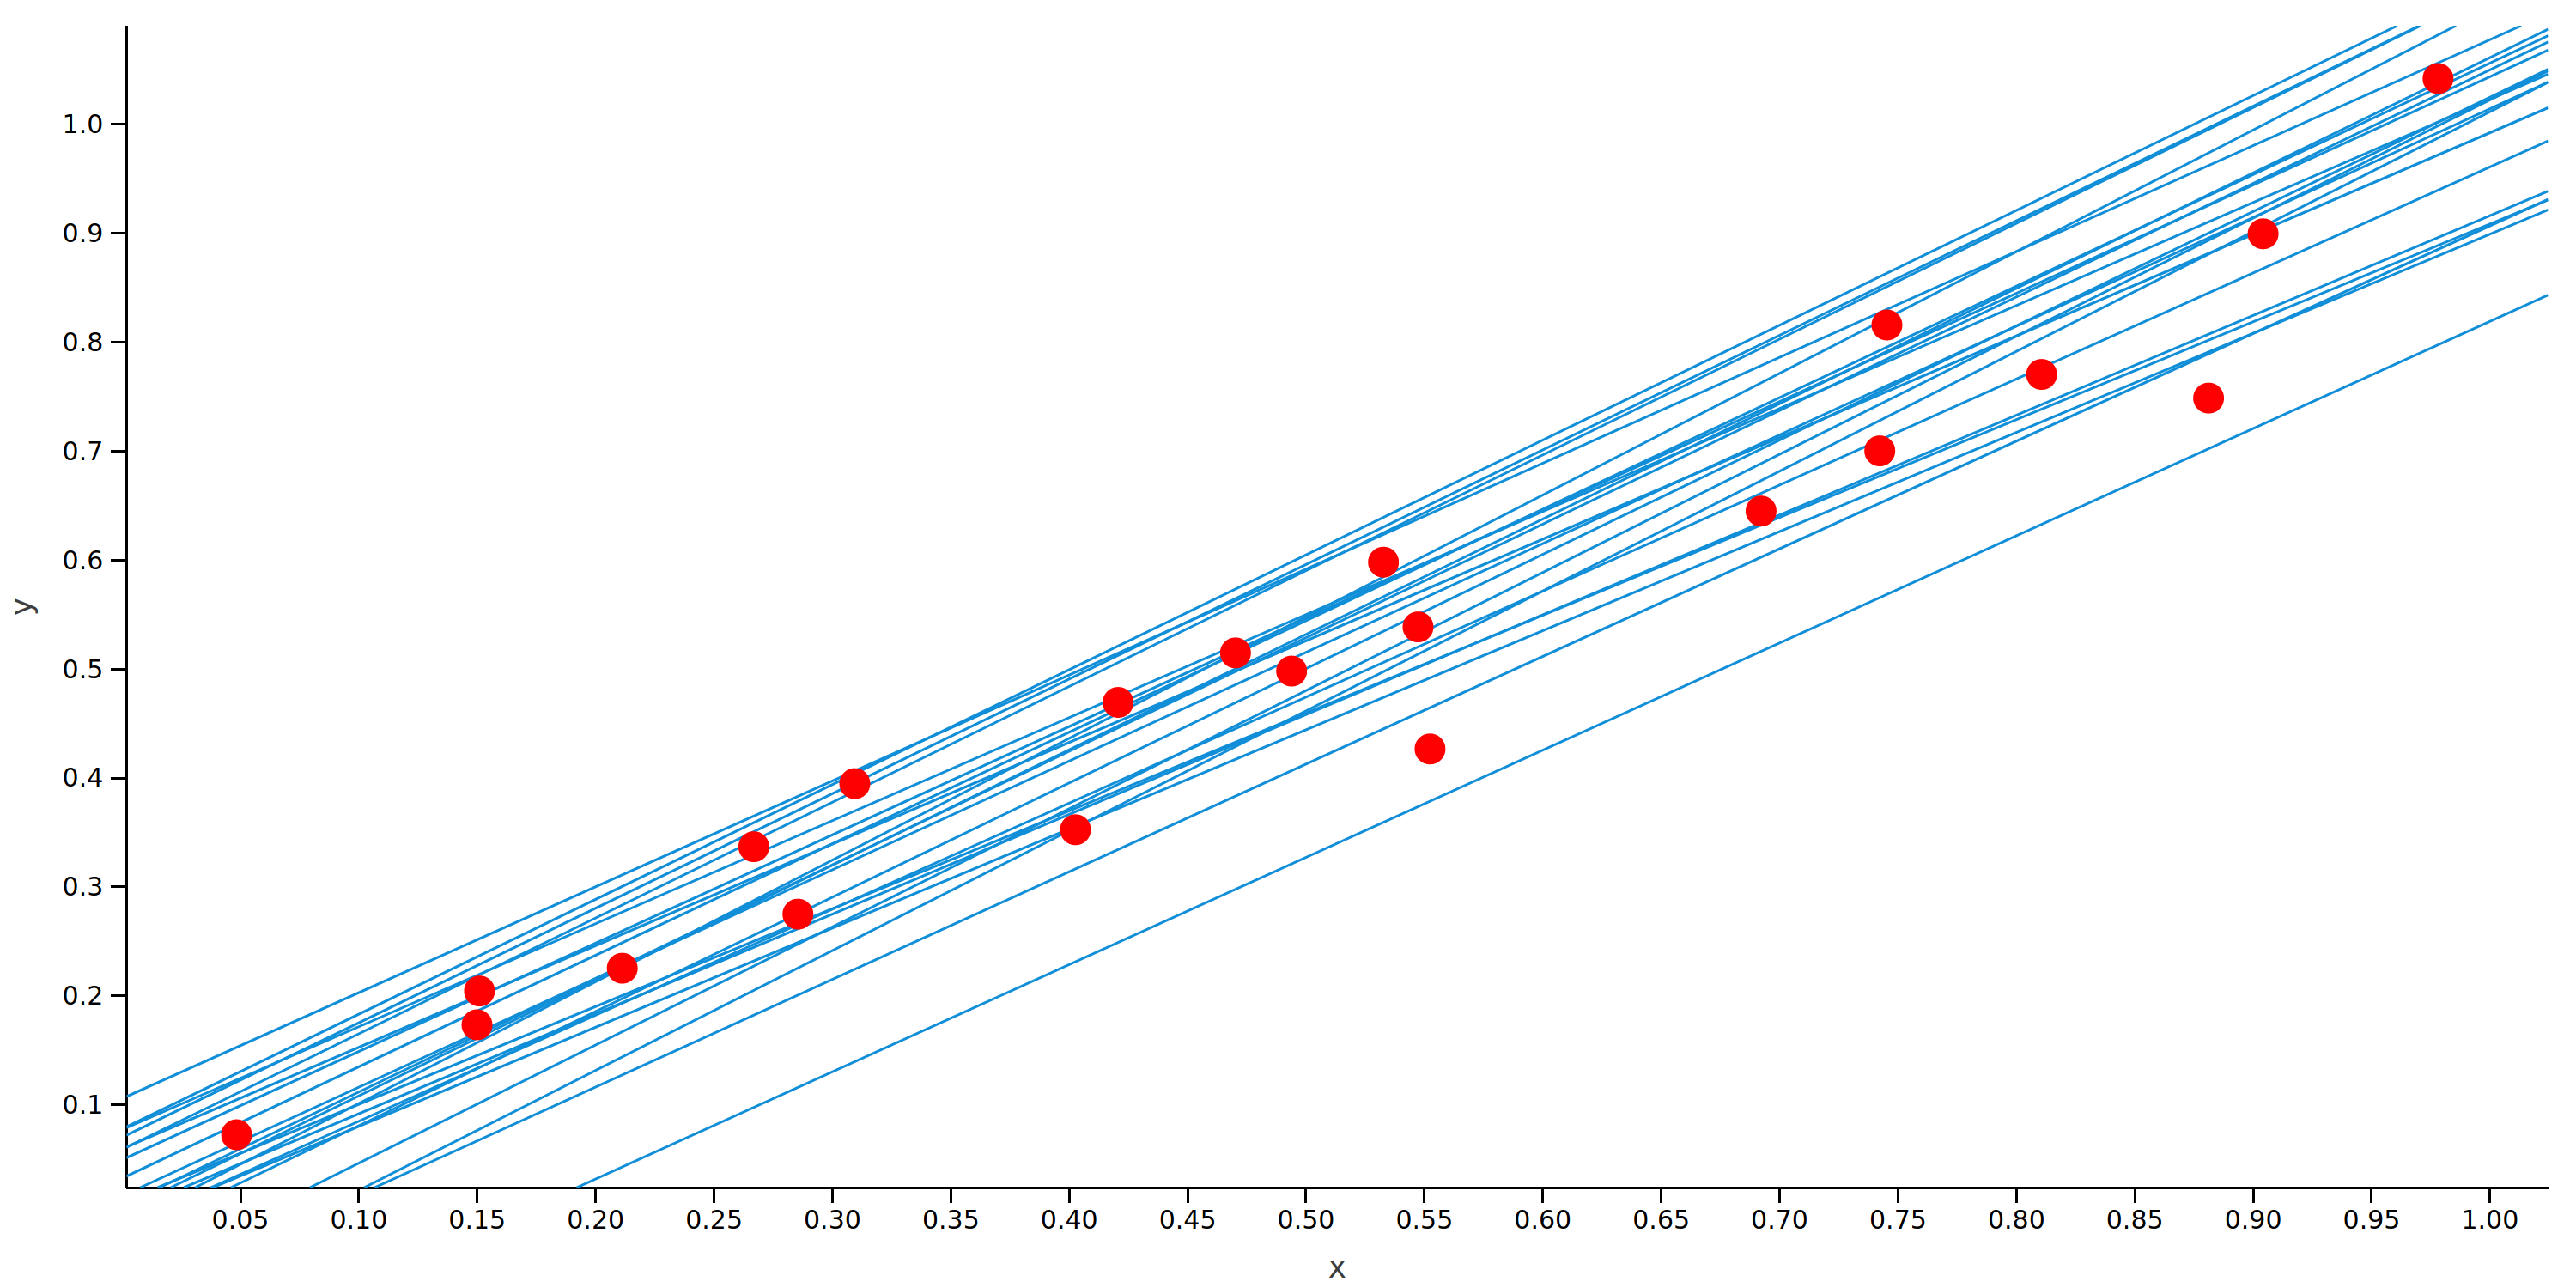
\includegraphics[width=\columnwidth]{bayesLR_plot.png}
Bayesian linear regression
\end{minipage}
&
\begin{minipage}[c]{0.5\columnwidth}
\centering
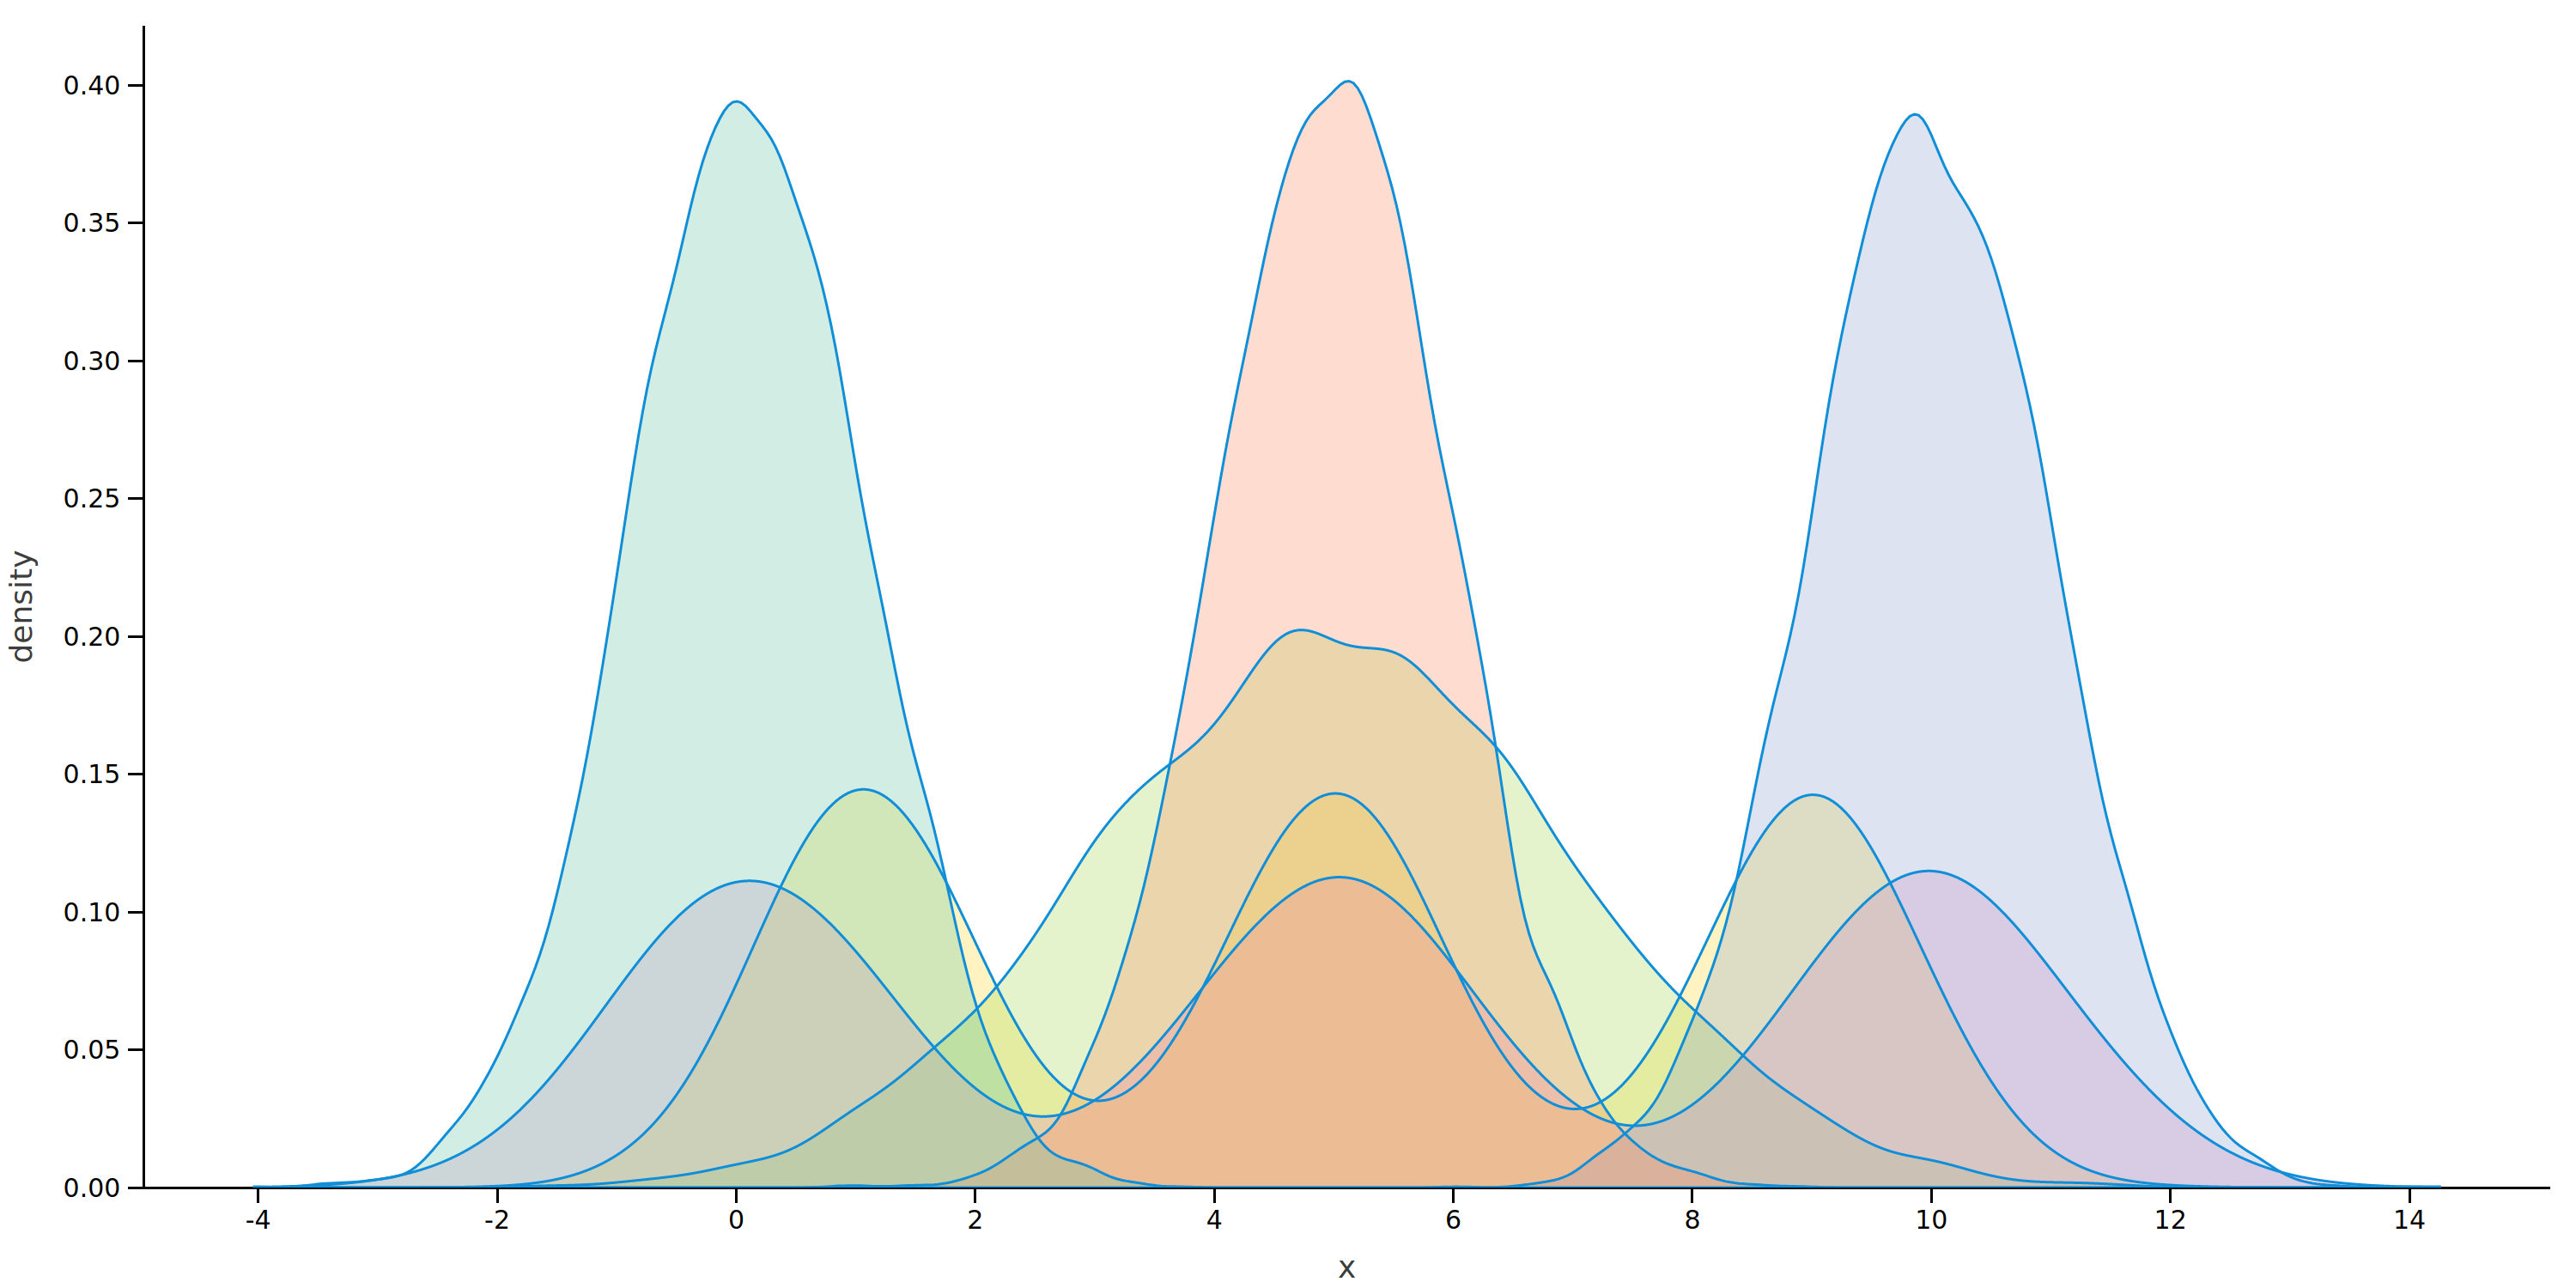
\includegraphics[width=\columnwidth]{plot.png}
Sum-product network
\end{minipage}
\end{tabular}

\vspace{\baselineskip}

We plan extend this DSL to support discriminative models and statistical inference.

\vspace{\baselineskip}

\mysection{Contributions}

\vspace{\baselineskip}

\begin{itemize}
  \item Lift numerical computation graph into the domain of probability kernels
  \item Implements general-purpose combinators for various probability distributions
  \item Implements domain-specific estimators for the algebra of random variables
  \item Allows flexible algebraic rewriting to optimize for e.g. latency or numerical stability
  \item Lowering to numerical values when necessary to perform e.g. sampling/inference
\end{itemize}

\vspace{\baselineskip}

\begin{tabular}{cc}
\begin{minipage}[c]{0.8\columnwidth}

Code available at: \url{https://github.com/breandan/markovian} \\

Paper available at: \url{https://brea.ndan.co/public/probcirc.pdf}
\end{minipage}
&
\begin{minipage}[c]{0.2\columnwidth}
\begin{centering}
\qrcode[height=2in]{kg.ndan.co}
\end{centering}
\end{minipage}
\end{tabular}

%\small{
%\bibliographystyle{unsrt}
%\bibliographystyle{../misc/natbib}
%\bibliography{../misc/library,../misc/biblio,../misc/bibdesk-porbanz}
%}

\end{multicols}

\end{poster}

\end{document}
